\chapter{ОБЗОР ОСНОВНЫХ ПОДХОДОВ ДЛЯ РЕАЛИЗАЦИИ МИКРОСЕРВИСОВ}
\section{Обзор микросервисной архитектуры}

Представление о микросервисах родилось в 2005 году из подхода SOA путем обобщения философии UNIX для веб-компонент.
Веб-сервисы сопоставляются независимым программам, комбинация которых осуществляется с помощью сетевого транспорта данных по аналогии с именованными и неименованными UNIX каналами.
В отличие от SOA микросервисы не фокусируются на конкретных форматах передачи данных, как SOAP, 
а дают представление о том, как должны коммуницировать сервисы, чтобы при сохранении слабой связности компонент поддерживать устоявшийся контракт обмена информацией \cite{micro-1}.

В современной литературе не существует одного конкретного определения микросервиса. 
Обычно микросервисы определяют через различные критерии соответствия распределенной системе с низкой связностью ее отдельных компонент.

Большое внимание в теории микросервисов уделяется вопросам масштабируемости. 
Для всестороннего описания масштабируемости в контексте разработки распределенных систем вводится понятие куба масшабируемости \cite{scalability} (Рисунок \ref{fig:cube}).

\begin{figure}[H]
    \centering
    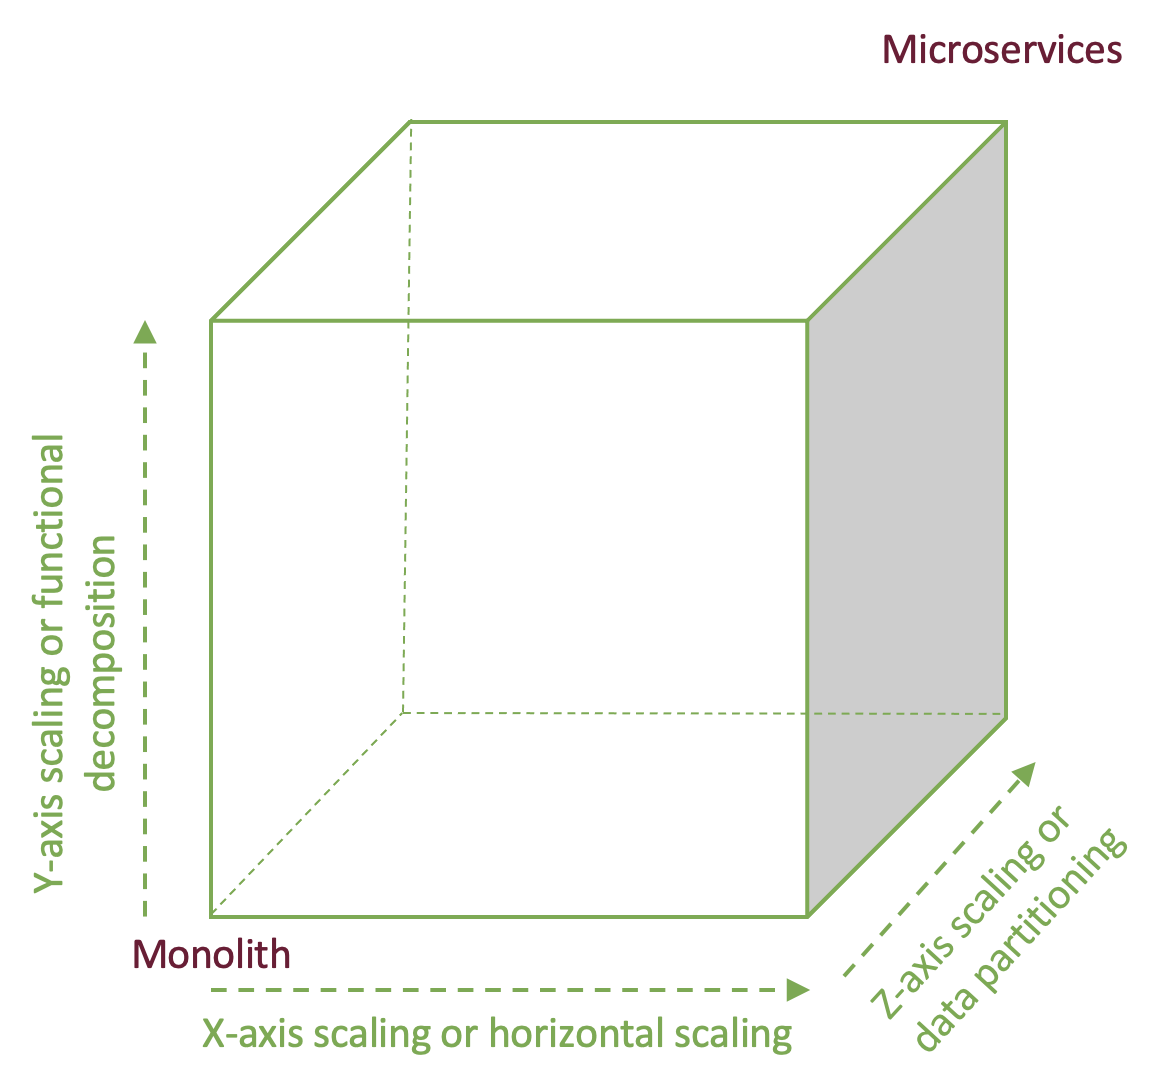
\includegraphics[width=0.4\linewidth]{img/cube.png}
    \caption{--- Куб масштабируемости}
    \label{fig:cube}
\end{figure}

Эта модель определяет три направления для масштабирования приложений: $X$, $Y$ и $Z$.

Масштабирование по оси X часто применяют в монолитных приложениях. 
Запускается несколько экземпляров программы, размещенных за балансировщиком нагрузки. 
Балансировщик распределяет запросы между $N$ одинаковыми экземплярами. 
Это распространенный способ улучшить
производительность и стабильность приложения.

Масштабирование по оси $Z$ тоже предусматривает запуск нескольких экземпляров
монолитного приложения, но в этом случае, в отличие от масштабирования по
оси $X$, каждый экземпляр отвечает за определенное подмножество данных.
Маршрутизатор, выставленный впереди, задействует атрибут запроса, чтобы на
править его к подходящему экземпляру. 

Масштабирование по осям $X$ и $Z$ увеличивает производительность и стабильность приложения.
Но ни один из этих подходов не решает проблем с усложнением кода и процесса раз
работки. Чтобы справиться с ними, следует применить масштабирование по оси $Y$,
или функциональную декомпозицию. То, как это работает, показано на рисунке \ref{fig:y}.
\begin{figure}[H]
    \centering
    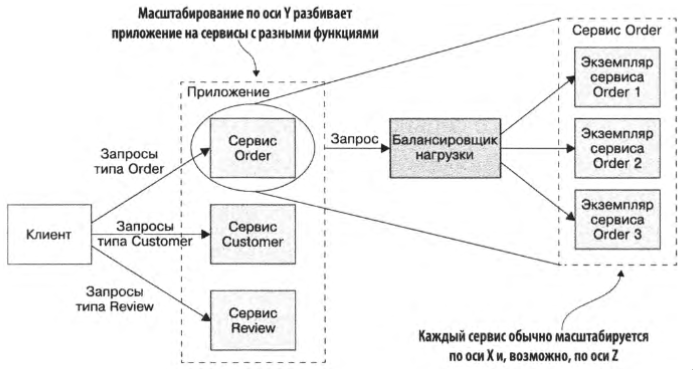
\includegraphics[width=0.8\linewidth]{img/y.png}
    \caption{--- Пример декомпозиции приложения через отдельные сервисы}
    \label{fig:y}
\end{figure}

Таким образом, сервис — это приложение, реализующее узкоспециализированные функции, такие как управление заказами, управление клиентами и т. д. 
Сервисы масштабируются по оси $X$, некоторые из них могут использовать также ось $Z$. Например,
сервис Order (Рисунок \ref{fig:y}) имеет несколько копий, нагрузка на которые балансируется.
Одно из обобщенных определение микросервисной архитектуры (или микросервисов)
звучит так: это стиль проектирования, который разбивает приложение на отдельные
сервисы с разными функциями. Заметим, что размер здесь вообще не упоминается.
Главное, чтобы каждый сервис имел четкий перечень связанных между собой обязанностей.

Микросервисная архитектура имеет следующие преимущества:
\begin{itemize}
    \item Она делает возможными непрерывные доставку и развертывание крупных, сложных приложений.
    \item Сервисы получаются небольшими и простыми в обслуживании.
    \item Сервисы развертываются независимо друг от друга.
    \item Сервисы масштабируются независимо друг от друга.
    \item Микросервисная архитектура обеспечивает автономность команд разработчиков.
    \item Она позволяет экспериментировать и внедрять новые технологии.
    \item В ней лучше изолированы неполадки других сервисов.
\end{itemize}

Одна из проблем, возникающих при использовании микросервисной архитектуры, связана с отсутствием конкретного, хорошо описанного алгоритма разбиения
системы на микросервисы. 
Что означает, что эта часть данной методологии, не имеет формального описания \cite{micro-1}. 

В связи с этим также выделяют понятие распределенного монолита.

Распределенным монолитом называют набор связанных между собой сервисов, которые необходимо развертывать вместе. Распределенному монолиту присущи недостатки
как монолитной, так и микросервисной архитектуры.

Еще один недостаток микросервисной архитектуры состоит в том, что при создании
распределенных систем возникают дополнительные сложности для разработчиков. 
Сервисы должны использовать механизм межпроцессного взаимодействия.

Это сложнее, чем вызывать обычные методы в общей памяти приложения. 
К тому же код должен уметь
справляться с частичными сбоями и быть готовым к недоступности или высокой
латентности удаленного сервиса.
Реализация сценариев, охватывающих несколько сервисов, требует применения
дополнительных технологий. 

\section{Практики использования СУБД в микросервисных архитектурах}

Для реализации надлежащего уровня изоляции между микросервисами применяется паттерн database per service.
В этом случае каждый микросервис имеет собственную базу данных при необходимости холодного хранилища данных. 
Это позволяет вносить правки в функциональность сервиса без риска сломать функциональность другого сервиса и привлечения других команд для согласования изменений, 
а также позволяет просто оценивать время ответов и нагрузку для каждого из сервисов по отдельности, что сложно осуществимо при использовании общих ресурсов.

Несмотря на вышеперечисленные преимущества упомянутого паттерна, database per service затрудняет реализацию комбинированных транзакций и запросов. 
Подобные операции по модификации данных в разных экземплярах баз данных называют распределенными транзакциями.
Возникновение распределенных транзакций в архитектуре приложения налагает ограничения на повторные запросы и хеджирование и усложняет
применение практик по повышению надежности системы, поскольку при повторных неиндемпотентных запросах или прерванных запросах на запись в несколько баз данных
может быть нарушена консистентность данных.
Для решения подобных проблем внедряются отдельные протоколы координации запросов в базы данных.

Примером подобного протокола является 2PC (two phase commit) -- двухфазный коммит. Этот протокол предполагает
наличие надежного координатора, который предоставляет общую точку синхронизации для разных сервисов, и откатывает изменения
во всех базах при возникновении ошибок в одном из узлов (Рисунок \ref{fig:twopc}).
\begin{figure}[H]
    \centering
    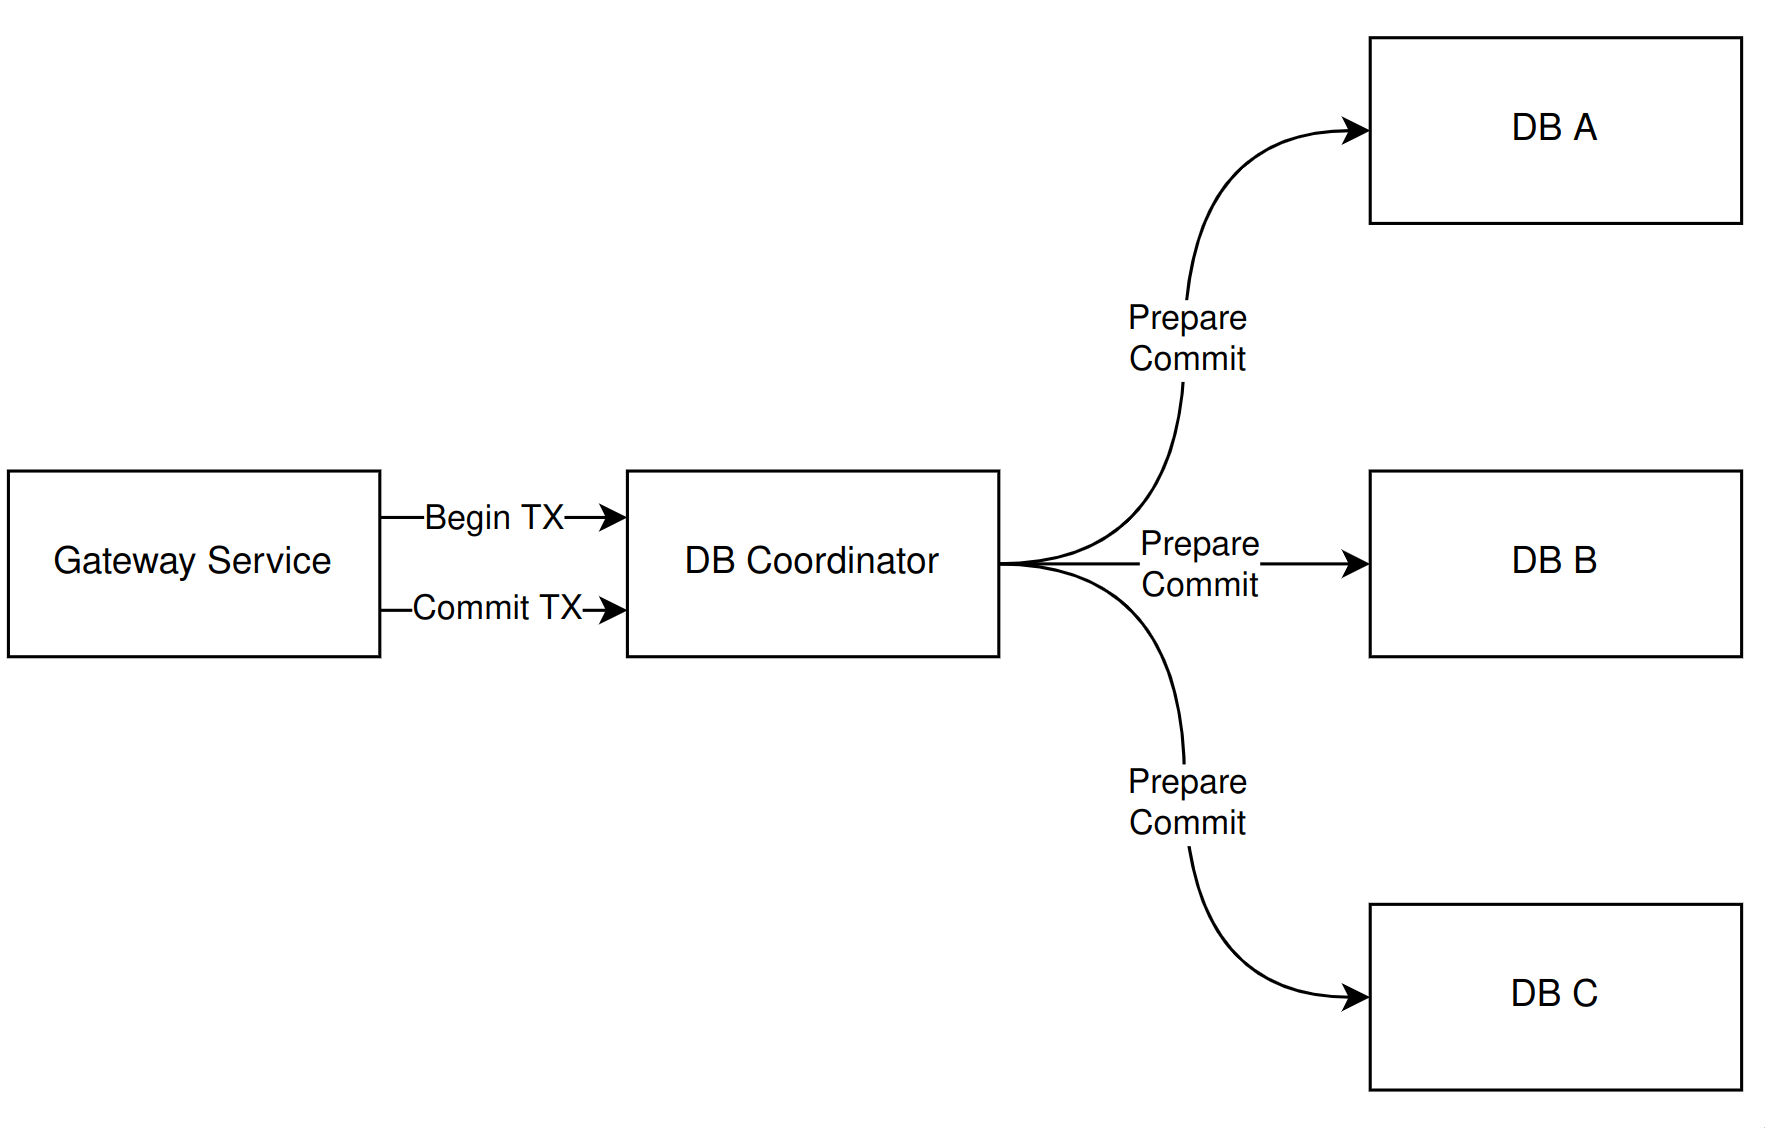
\includegraphics[width=0.8\linewidth]{img/2pc.png}
    \caption{--- Принцип работы 2PC}
    \label{fig:twopc}
\end{figure}

Несмотря на то, что протокол был разработан в 70-ые годы, он до сих используется в современных приложениях, например,
с помощью менеджера транзакций Narayana для платформы Spring. Многие базы данных также предоставляют достаточные механизмы транзакций, которые
требуются для реализации данного протокола. Подобные транзакции называют XA (Extend Architecture) транзакциями, которые обеспечивают
консистентность данных за счет дополнительной синхронизации.
В данном случае достигается максимально возможная консистентность данных, однако
необходимость в отдельном узле синхронизации снижает производительность, усложняет масштабирование из-за ограничений координатора, и конфигурация подобных систем
может быть довольно сложной.
Также данный протокол плохо применяется
для нереляционных баз данных, что неприемлемо для современных приложений.

Для решения вышеперечисленных проблем прибегают к паттерну Saga. В этом случае в качестве координатора
выступает один из сервисов (Рисунок \ref{fig:saga}), который осуществляет модификацию данных в других сервисах в рамках своих транзакций.
При возникновении ошибок на такой сервис-оркестратор возлагается ответственность вызвать нужные методы
для попытки сохранить или восстановить консистентность данных в других базах.

\begin{figure}[H]
    \centering
    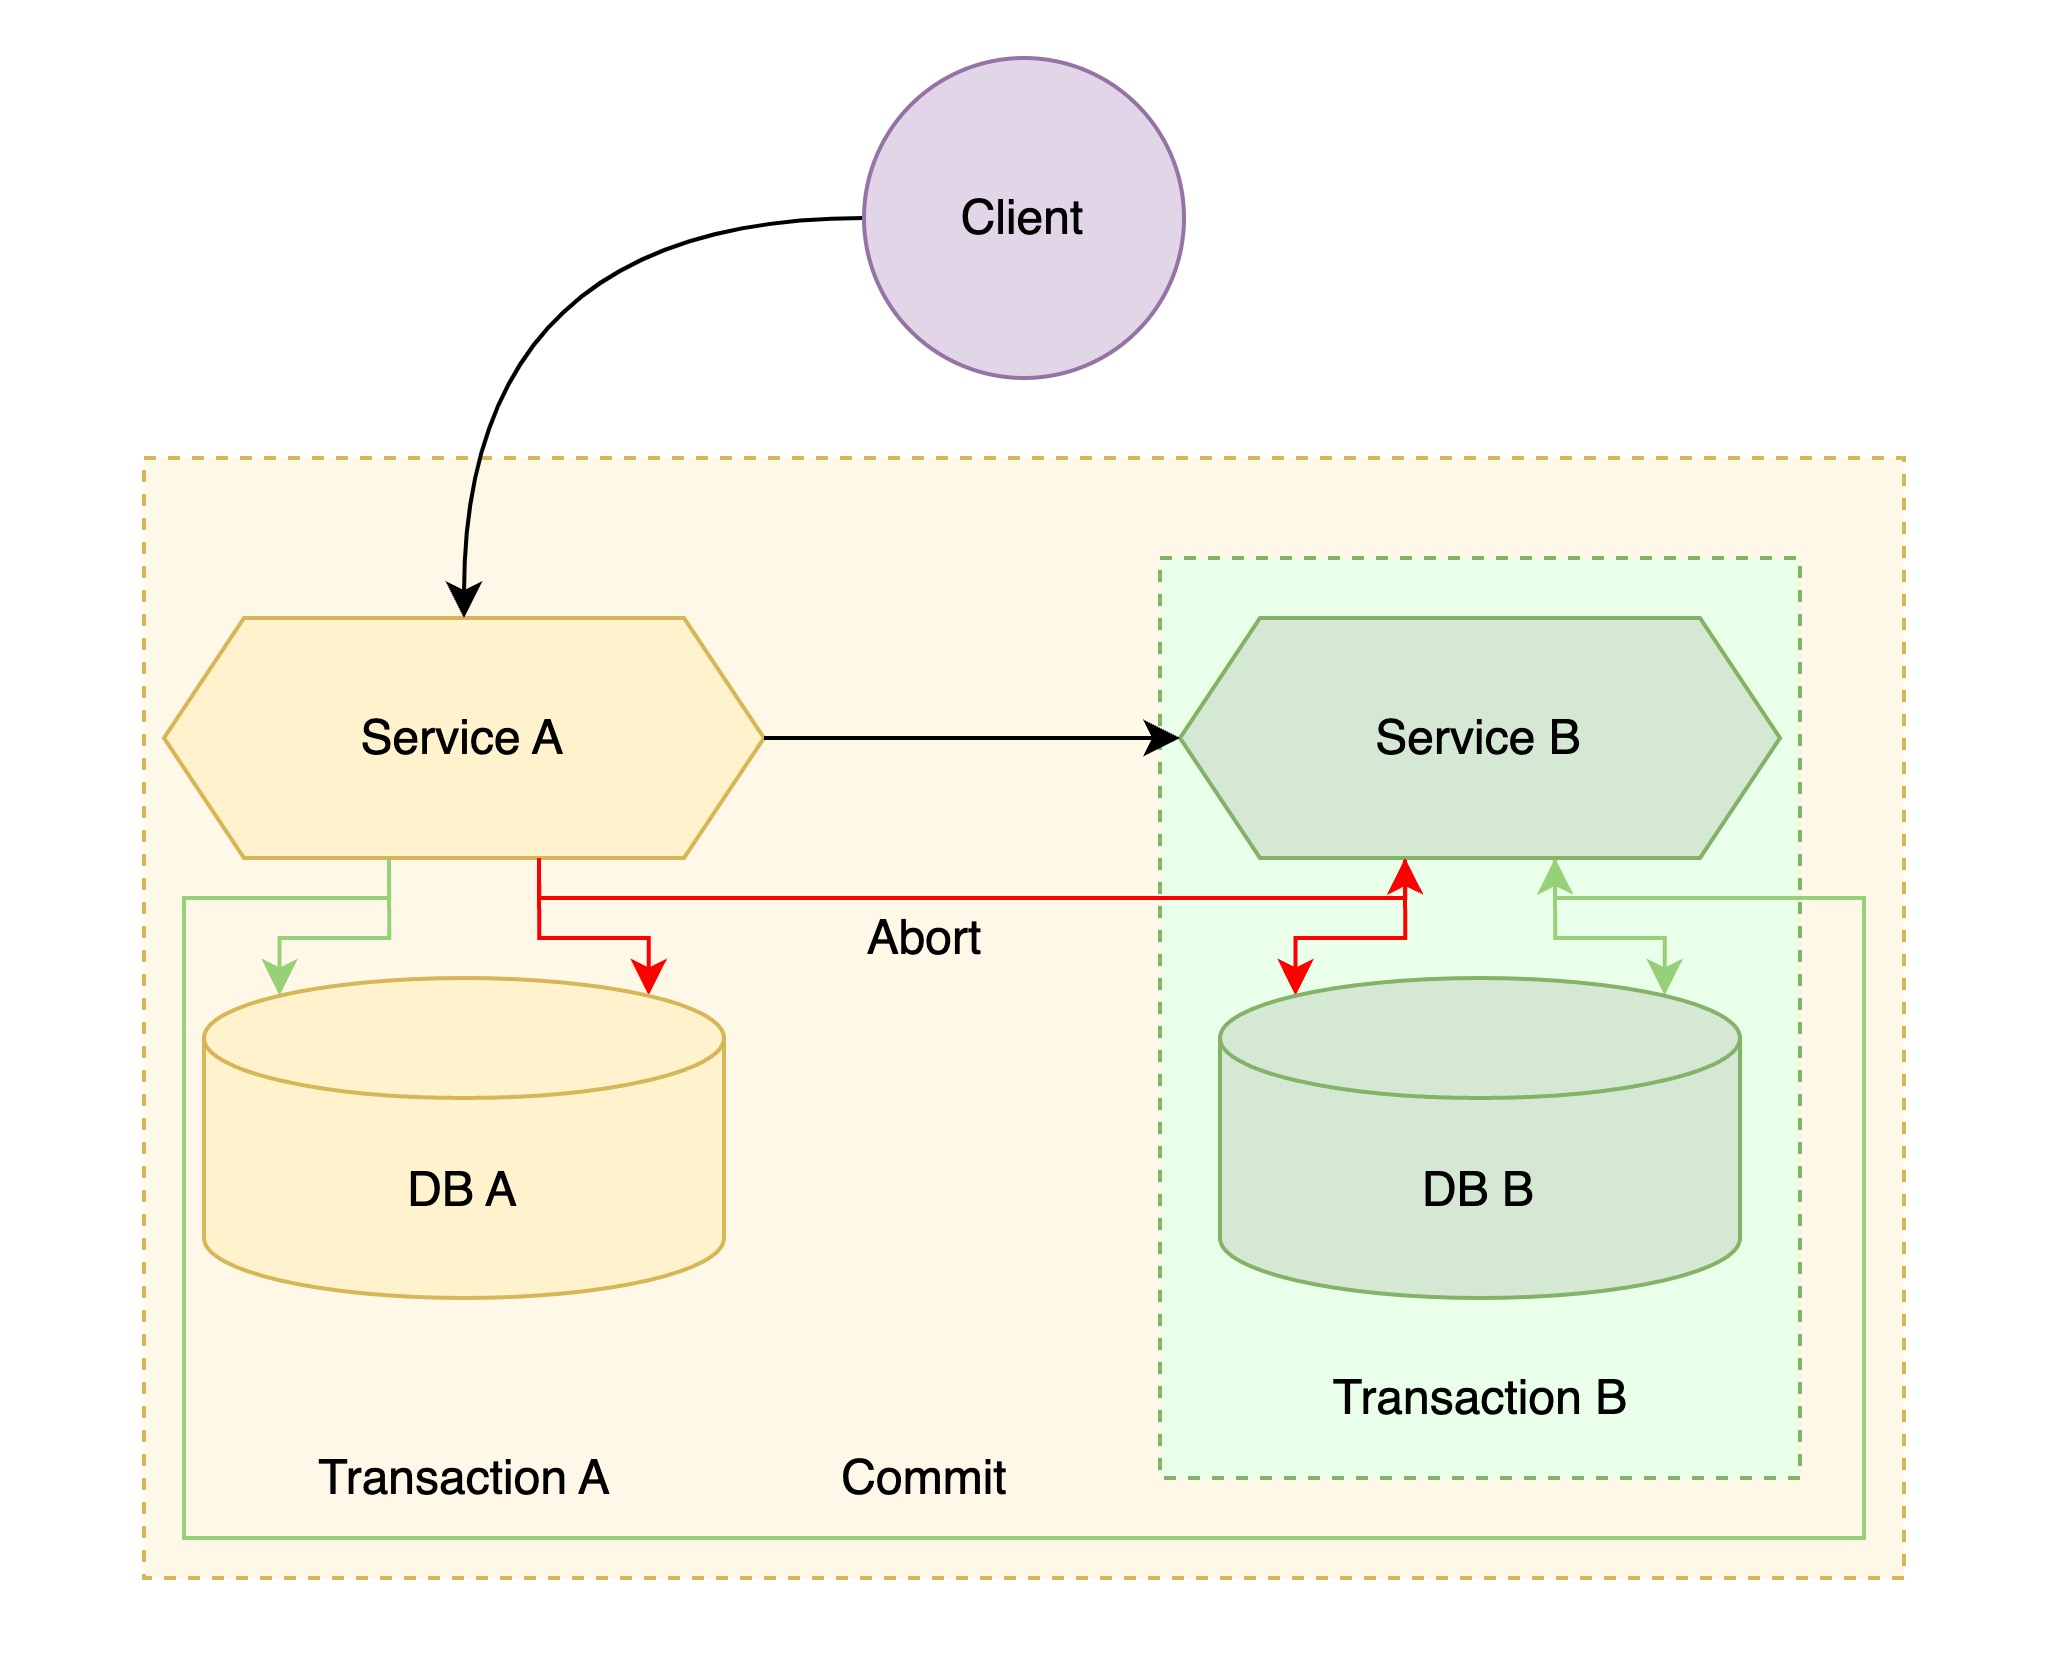
\includegraphics[width=0.8\linewidth]{img/saga.png}
    \caption{--- Принцип работы Saga}
    \label{fig:saga}
\end{figure}

При использовании одного из сервисов в качестве координатора уменьшаются задержки
коммуникации между сервисами и не требуются XA транзакции, что положительно сказывается на производительности
системы. Однако подобный подход не обеспечивает таких же гарантий консистентности данных, как 2PC или контроль над исполнением
транзакций в монолитном приложении. Поэтому может подойти для систем, где требования к производительности выше требований консистентности.

В качестве альтернативы также применют модификации Saga, где координатора может не быть вовсе. В этом
случае все операции модификации данных происходят асинхронно. Например, сервис, который раньше был координатором теперь может записывать
события, которые должны воспроизвести нужное состояние системы в отдельную очередь, которую читает другой сервис и самостоятельно управляет своими транзакциями.
В этом случае нет издержек на централизованное управление транзакций, а контроль над исполнением возлагается на механизмы обработки сообщений брокера (Рисунок \ref{fig:saga_async}).
Однако возникают проблемы с тем, что данные в базах данных больше не синхронизированы, 
и при отмене транзакции в одном сервисе после записи в очередь другой сервис может не получить об этом ответного сообщения.

\begin{figure}[H]
    \centering
    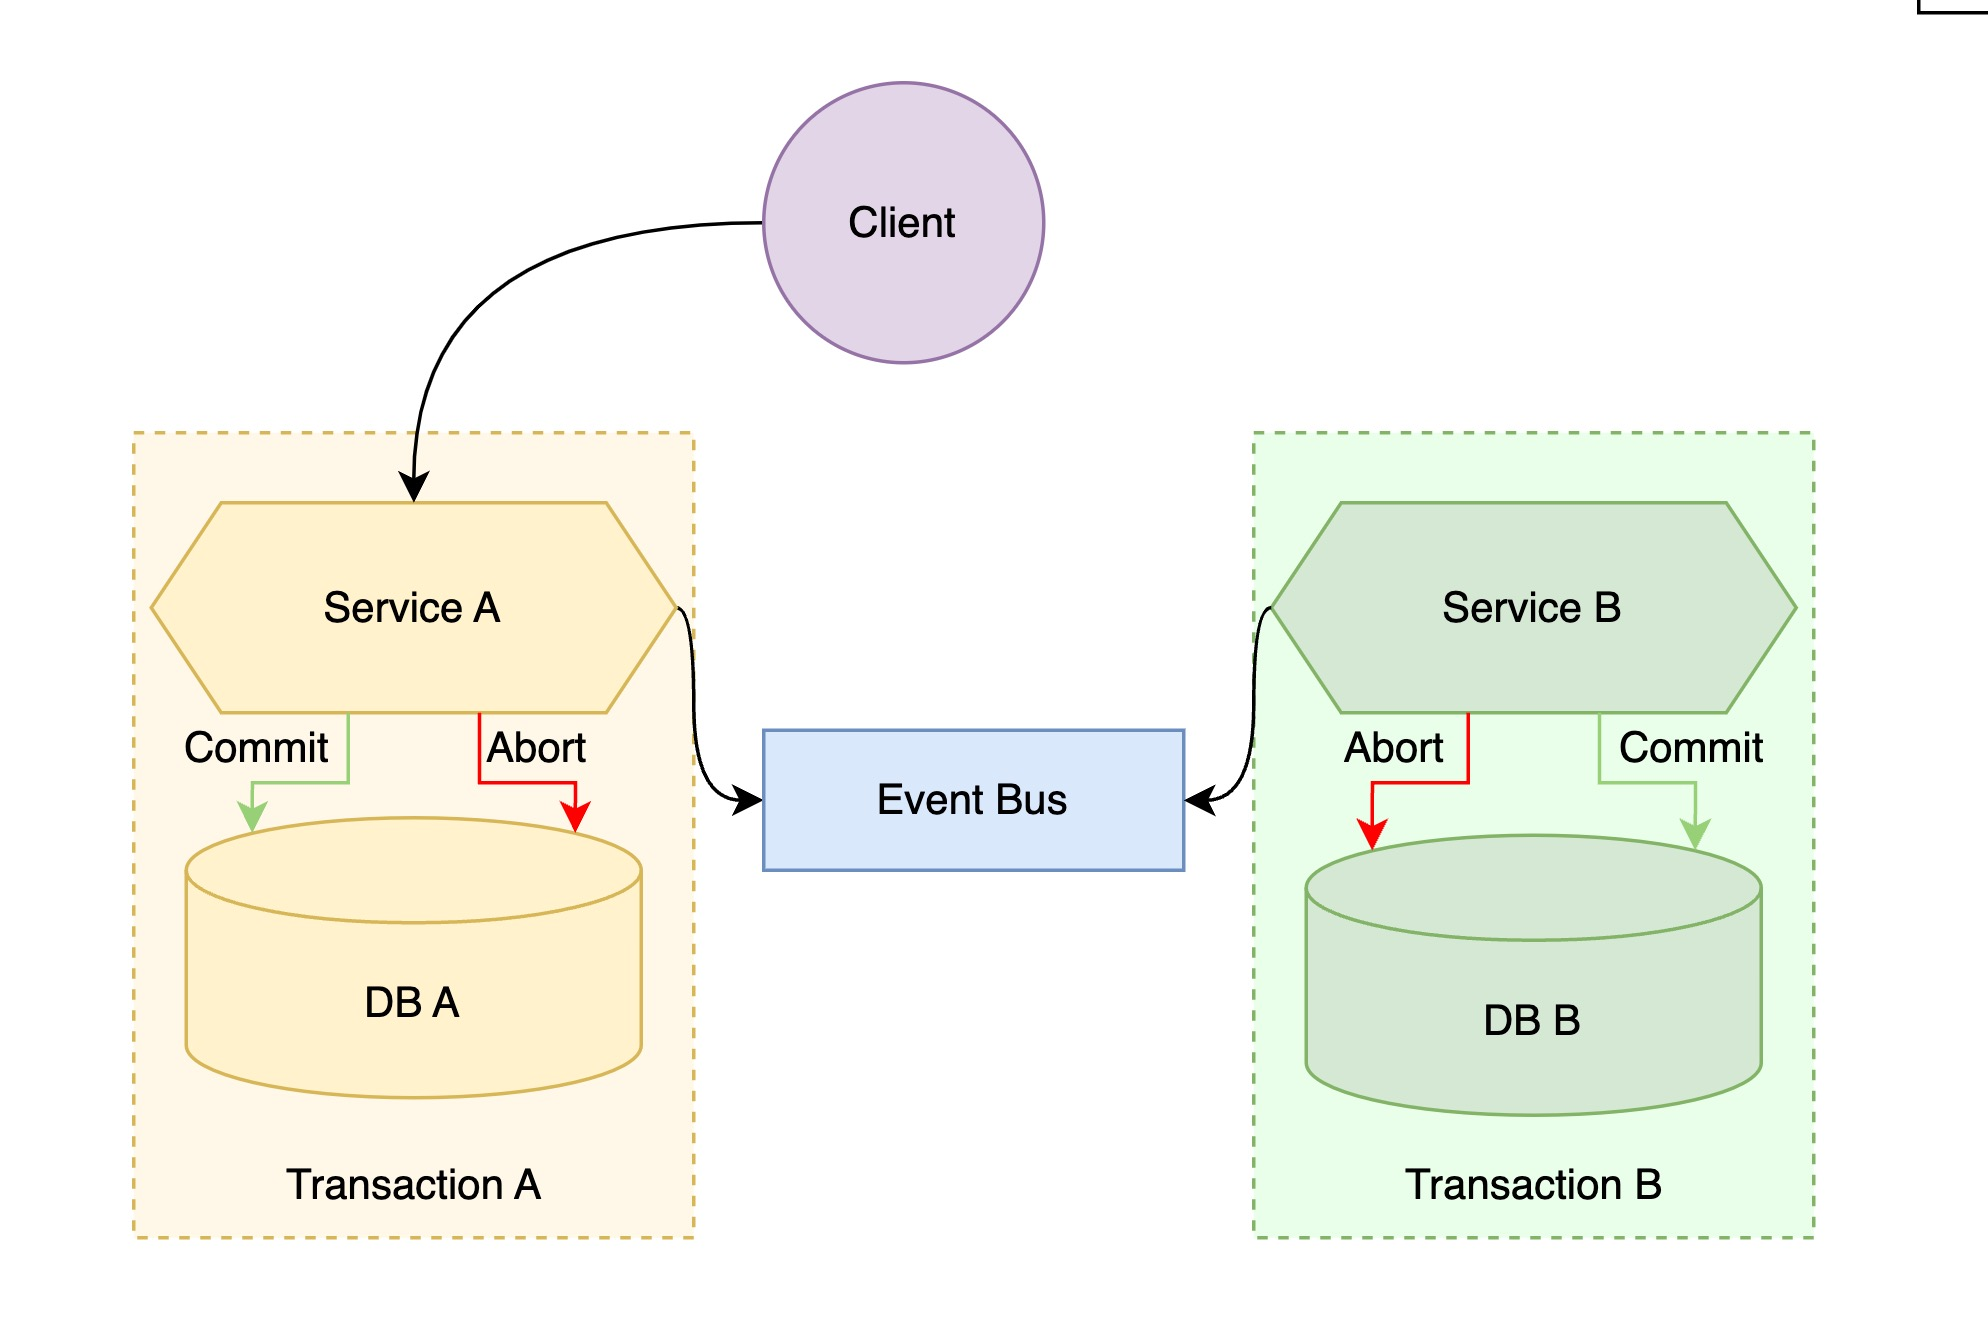
\includegraphics[width=0.8\linewidth]{img/saga_async.jpeg}
    \caption{--- Принцип работы Saga без централизованного координатора}
    \label{fig:saga_async}
\end{figure}

Поэтому иногда коммуникацию между сервисами осуществляют непосредственно через одну из баз данных, которую в асинхронном режиме
сканируют другие сервисы. Постоянное чтение всех данных в базе данных координаторе может вызвать проблемы с производительностью, поэтому 
стоит прибегать к механизмам потоков изменений, как например в YDB. Тем не менее, как было описано ранее, общий доступ в одну базу данных
считается антипатерном при разработке распределенных систем, поэтому не является рекомендуемым подходом.

\begin{figure}[H]
    \centering
    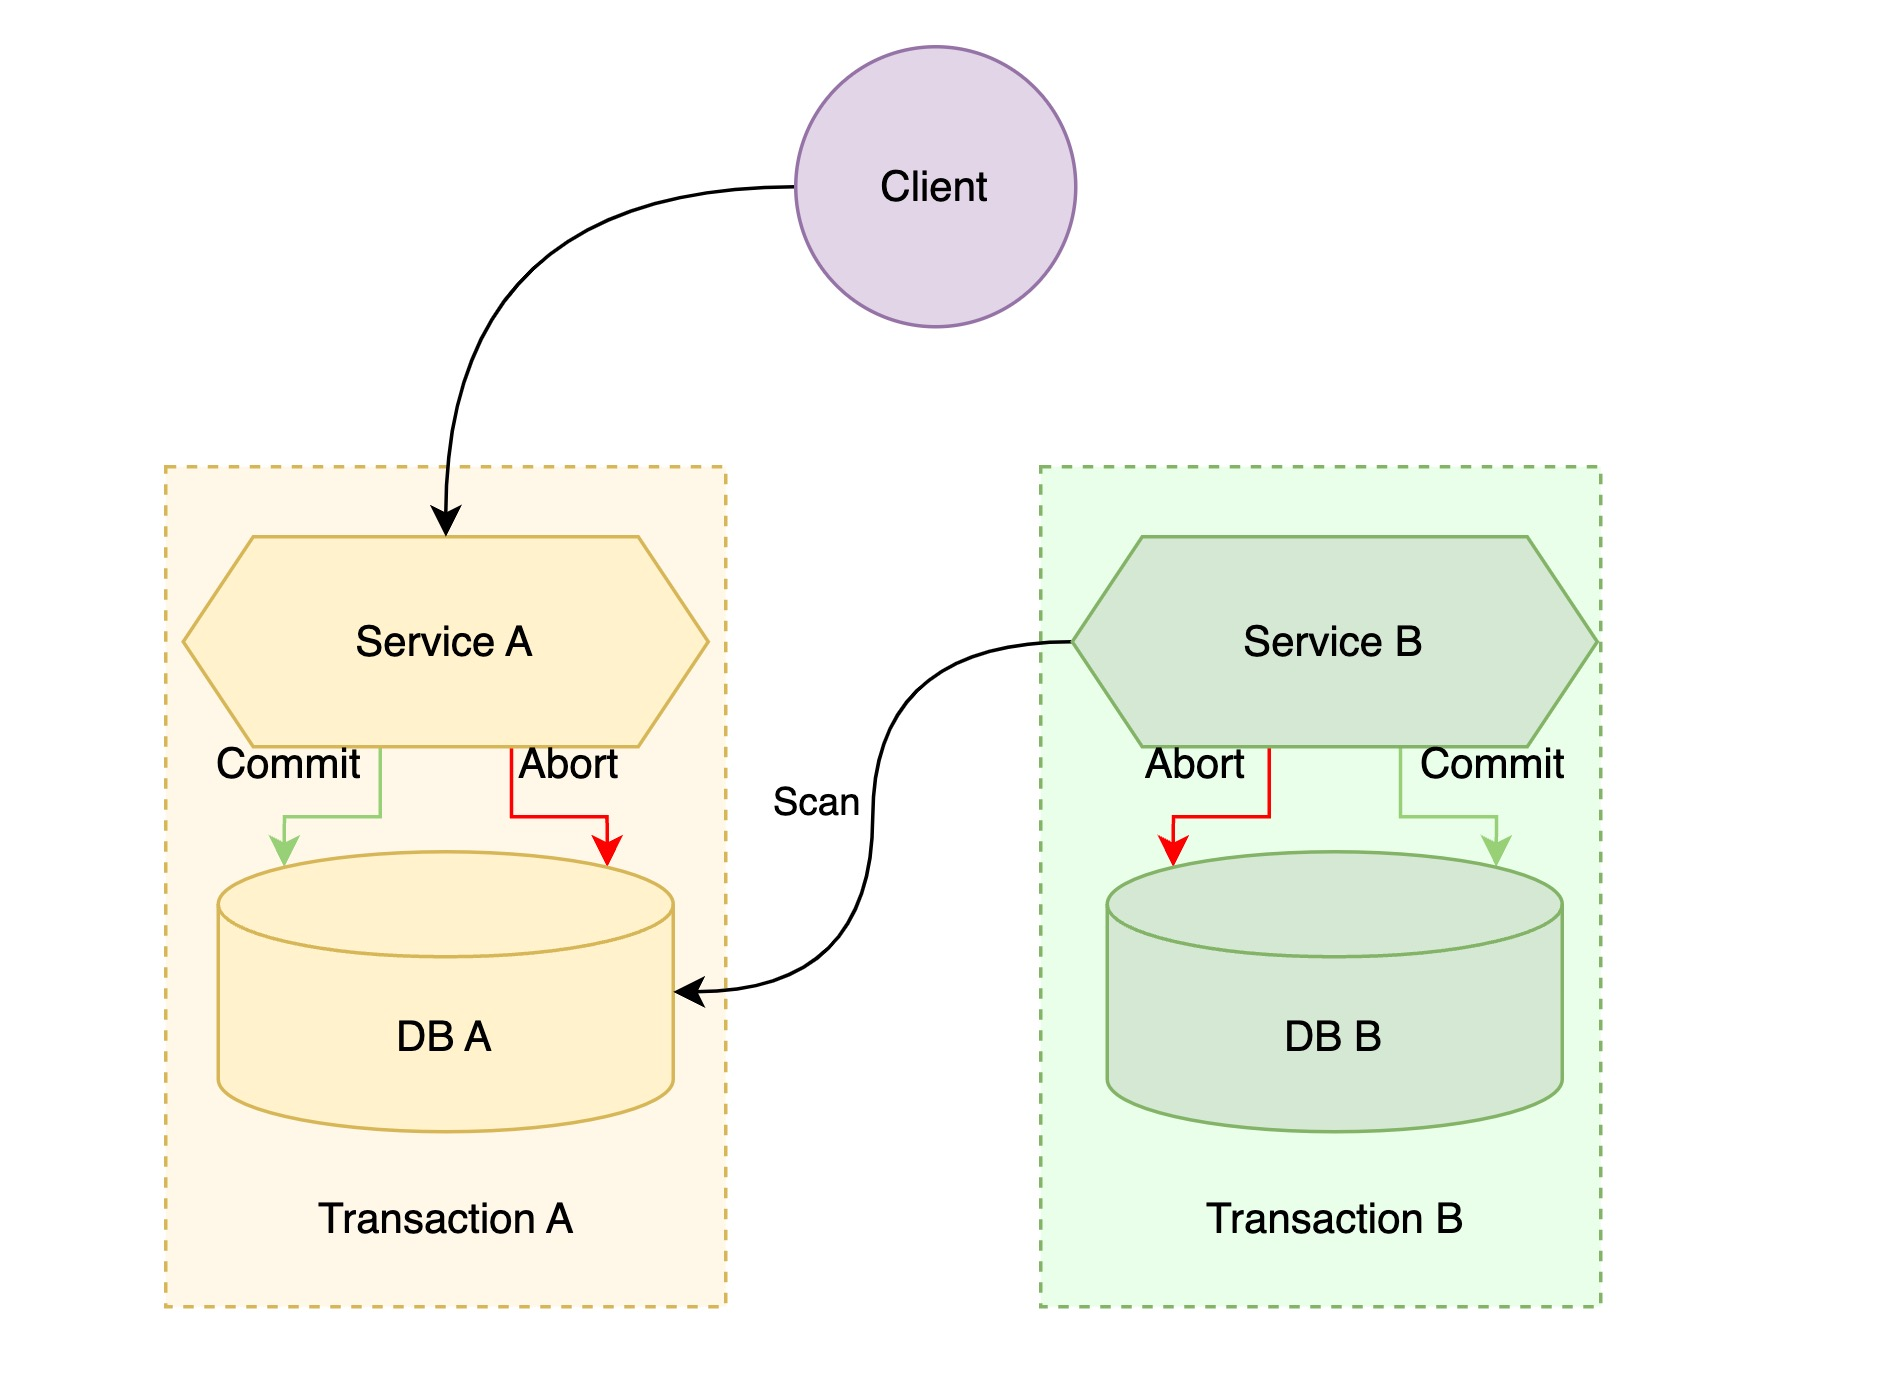
\includegraphics[width=0.8\linewidth]{img/saga_scan.jpeg}
    \caption{--- Принцип работы Saga с синхронизацией через одну из баз данных}
    \label{fig:saga_db}
\end{figure}

\section{Практики применения систем оркестрации в микросервисных архитектурах}
Внедрение микросервисной архитектуры также сопровождается вопросами релизного цикла и выкладки новых версий. Не всегда отдельные компоненты 
системы можно обновлять независимо, тогда как монолитные приложения можно обновлять без дополнительной координации, поскольку вся
система функционирует в рамках одного процесса. Поэтому при внедрении микросервисов стоит обратить особое внимание на системы оркестрации
и непрерывного деплоя, также называемого Green-blue деплоем. 

Green-blue деплой подразумевает совокупность стратегий по постепенной выкатке нового функционала. Одной из
самых распространенных систем оркестрации является Kubernetes, разработанный компанией Google.

Конкретно green-blue деплой реализуется через одномоментное переключение трафика из старых версий веб-приложения
в новые версии (Рисунок \ref{fig:gb}). Быстрое переключение трафика достигается за счет инструментов виртуализации, например, с помощью Docker-контейнеров,
которые содержат образ операционной системы, персистентное переиспользуемое хранилище данных из файловой системы и агенты виртуализации, которые
поддерживают связь с супервизором, который связывает контейнеры с io хостовой операционной системы.
Помимо быстрого переключения на новую версию приложения обеспечивается также возможность быстро откатить
примененные изменения, что является мощным средством предотвращения проблем, связанных с уязвимостями и багами
системы. 
\begin{figure}[H]
    \centering
    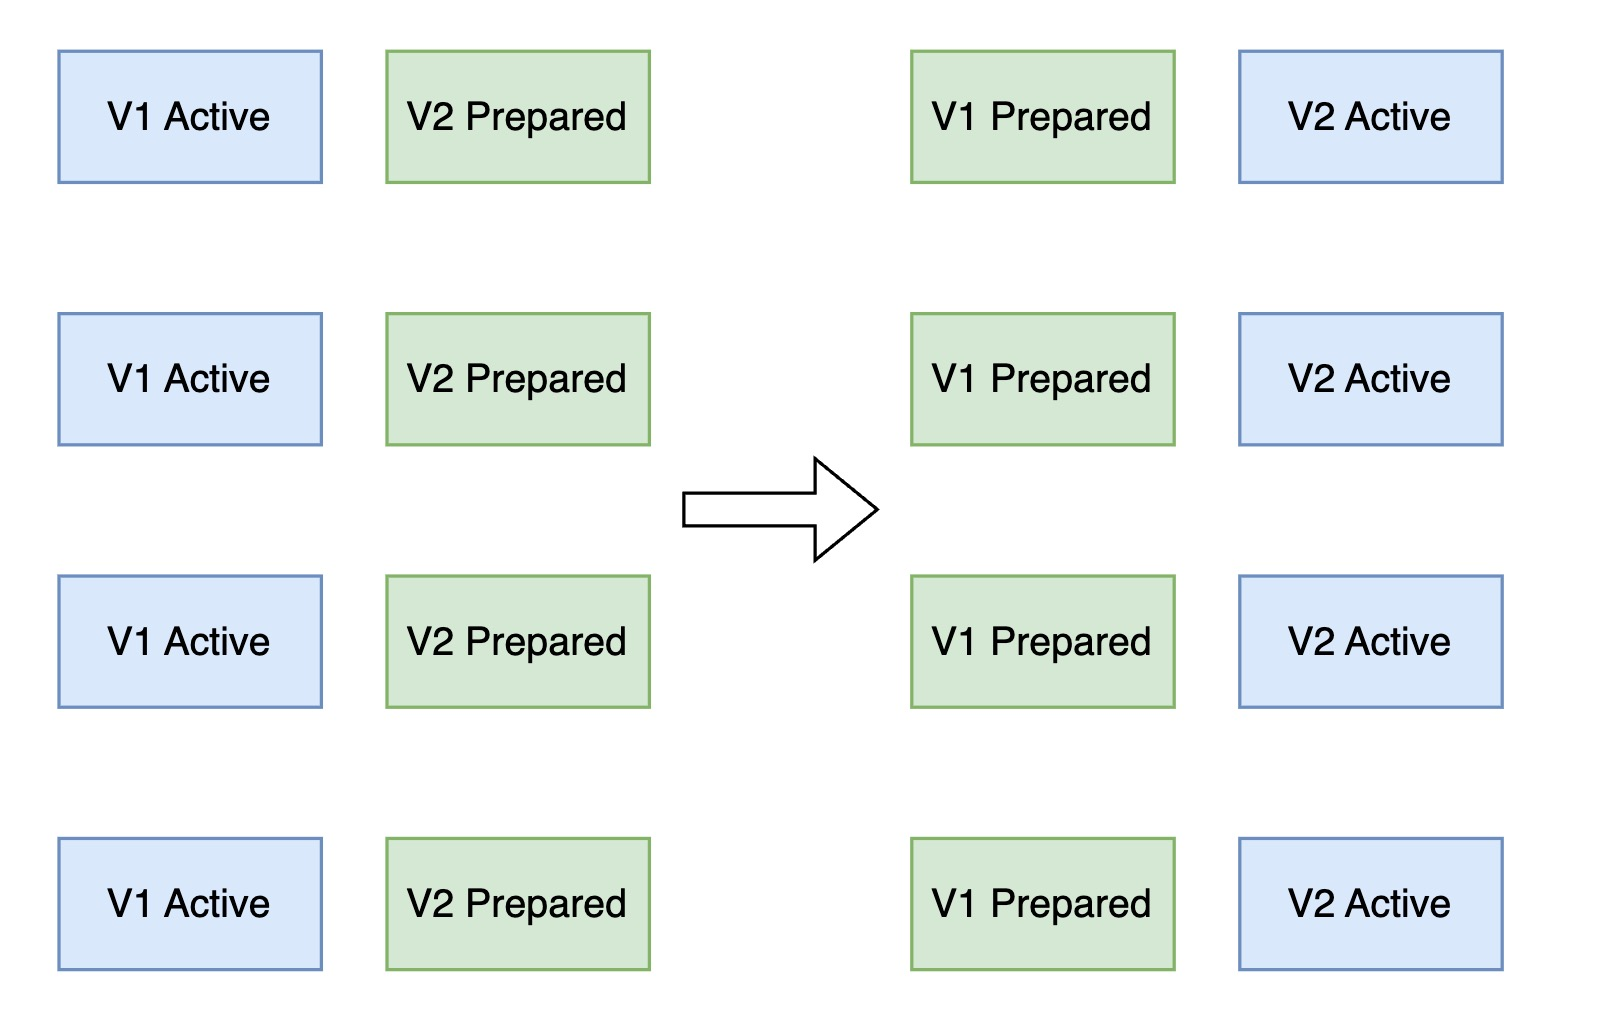
\includegraphics[width=0.8\linewidth]{img/gb.jpg}
    \caption{--- Процесс выкладки при green-blue развертывании}
    \label{fig:gb}
\end{figure}

Помимо green-blue деплоя применяются подходы, вроде rolling обновлений (Рисунок \ref{fig:rolling}), при которых обновление не происходит
одномоментно, а постепенно. В этом случае новая версия приложения также подготавливается заранее, и процесс обновления
постепенно переключает трафик со старых версий на новые.

\begin{figure}[H]
    \centering
    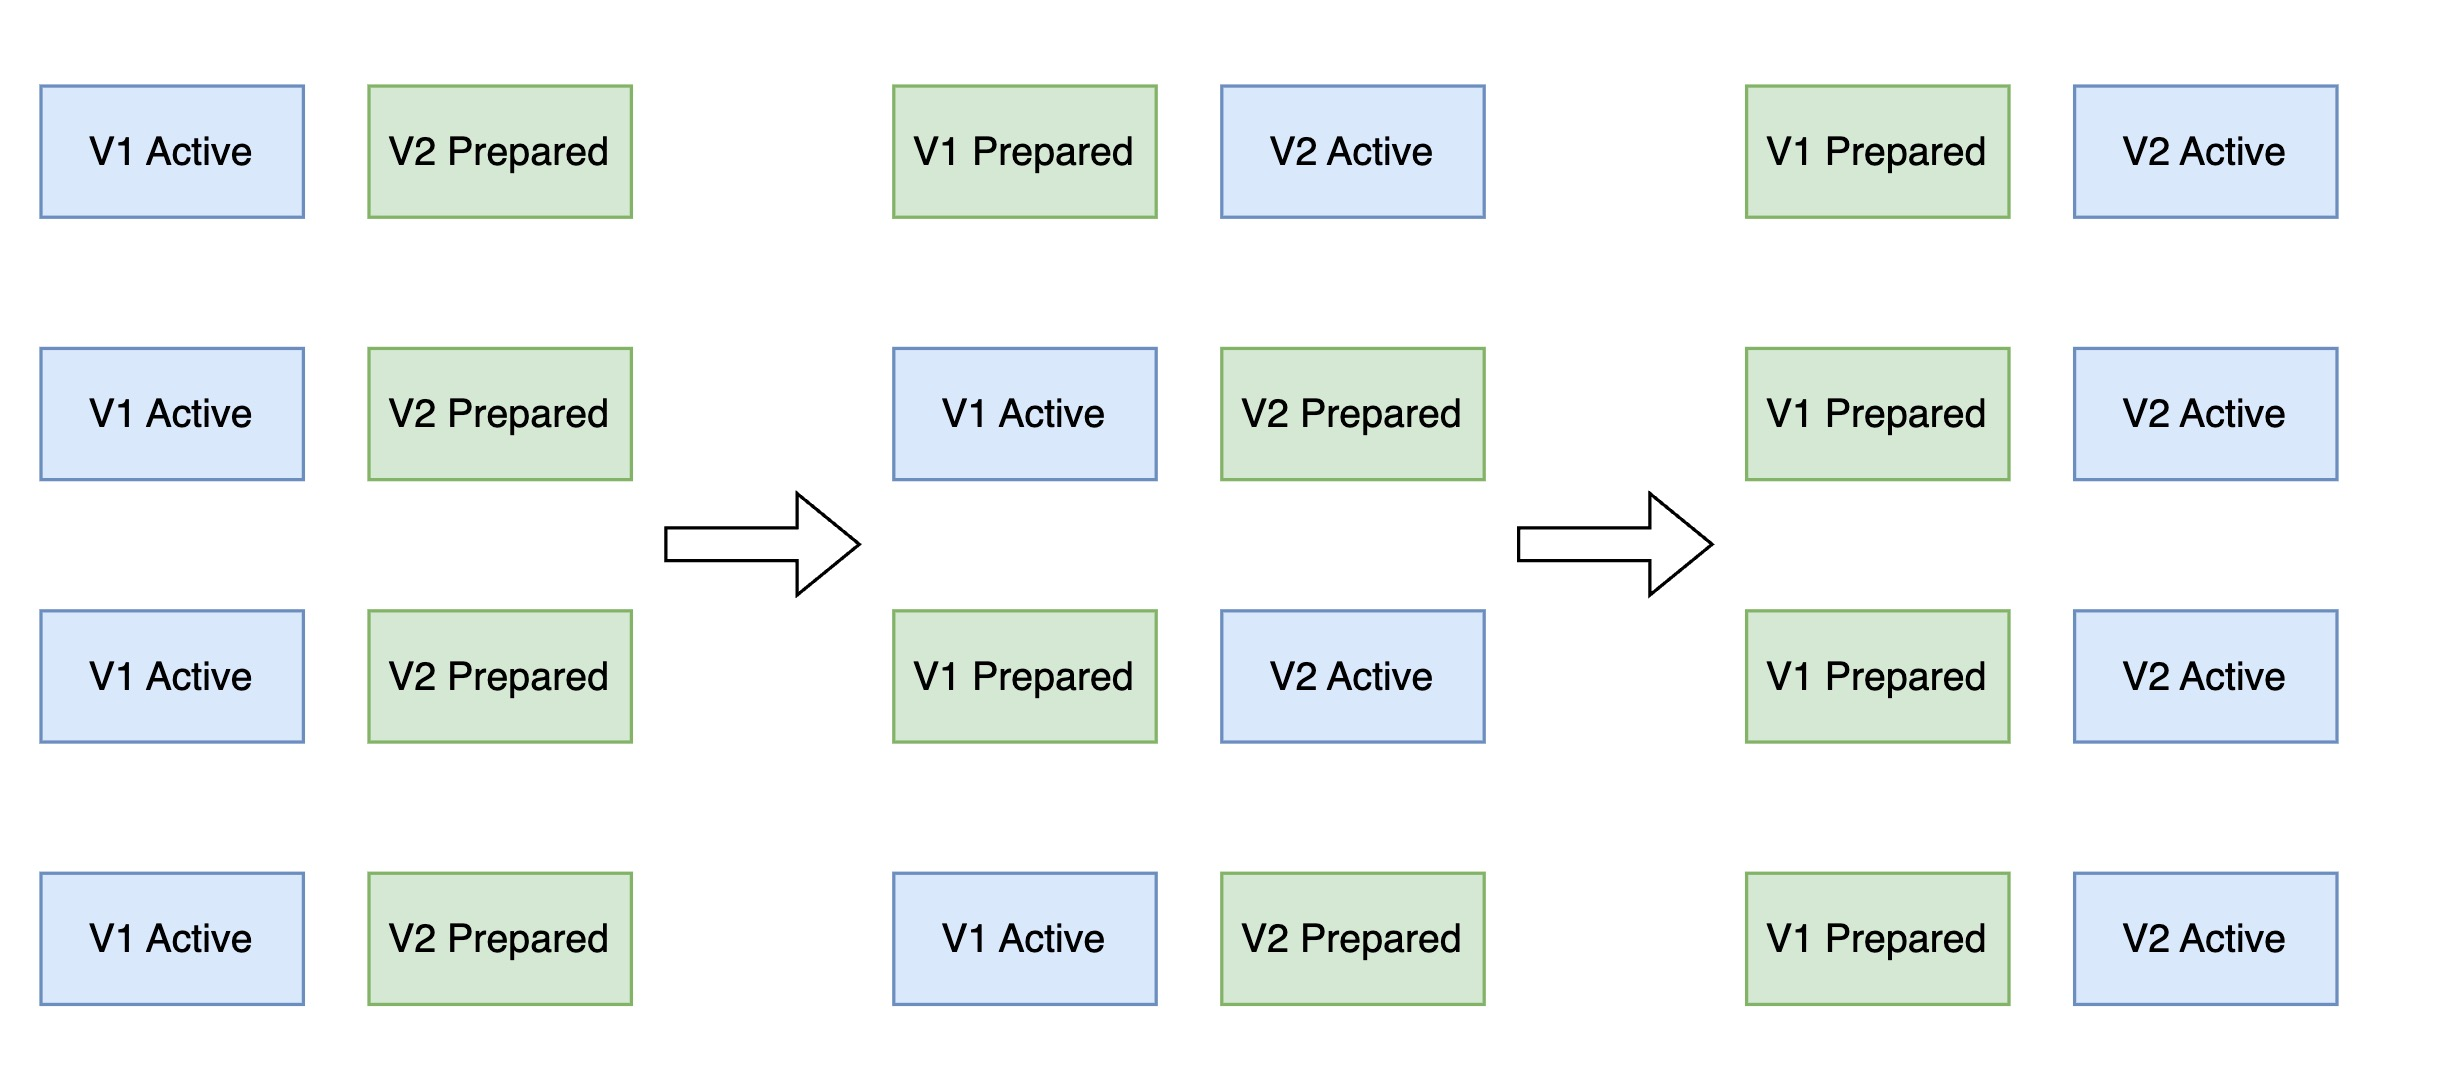
\includegraphics[width=0.8\linewidth]{img/rolling.jpg}
    \caption{--- Процесс выкладки при rolling развертывании}
    \label{fig:rolling}
\end{figure}

Для ранней диагностики проблем также может быть подготовлено отдельное окружение, называемое Canary или престабильным, которое дублирует или делит 
зависимости со стабильной версией, куда будет перенаправляться небольшой процент трафика от случайно выбранных или выбранных
по определенному признаку пользователей (Рисунок \ref{fig:canary}). Подобный подход зачастую применяется крупными компаниями, типа Netflix или Google, для
тестирования нового функционала на пользователях, что значительно упрощает последующую выкладку в стабильное окружение
и минимизирует риски. В подобном подходе помимо систем оркестрации требуется настройка 
сети на балансере прикладного уровня, который будет перенаправлять трафик Canary контур. 

\begin{figure}[H]
    \centering
    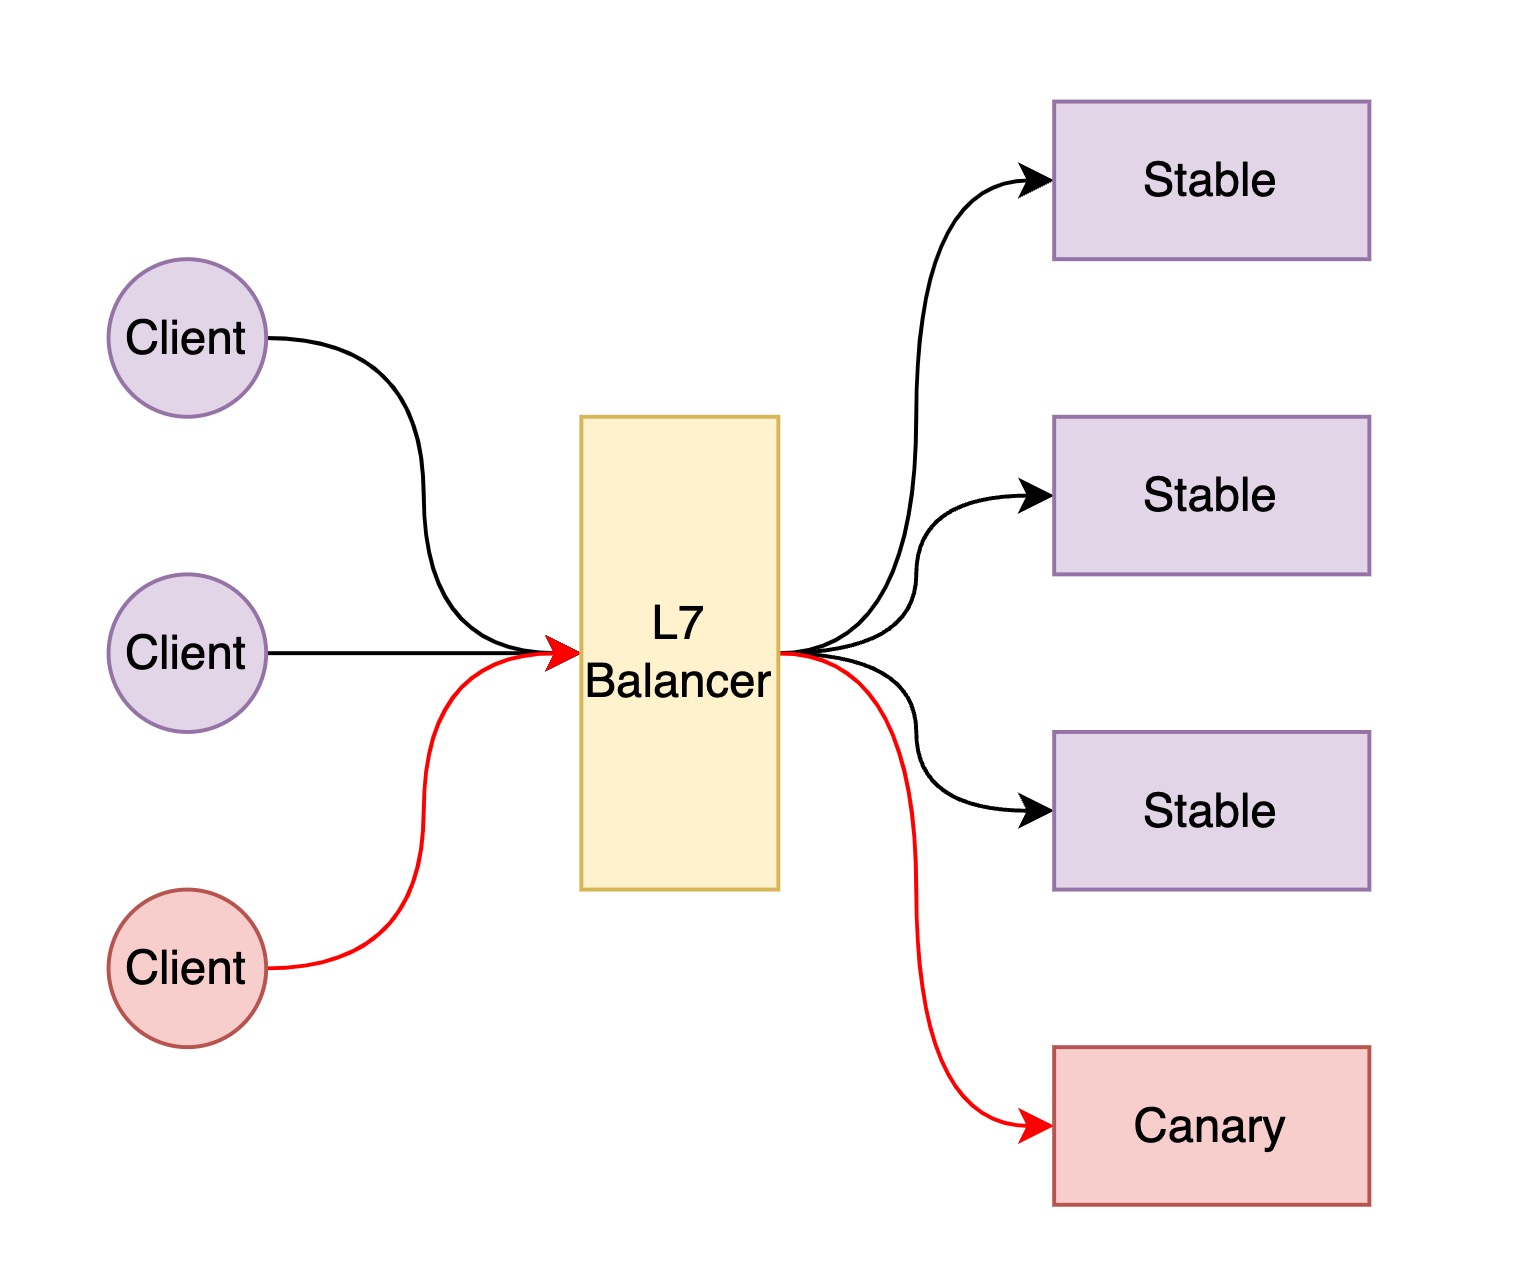
\includegraphics[width=0.8\linewidth]{img/canary.jpg}
    \caption{---  Процесс развертывания c Canary контуром}
    \label{fig:canary}
\end{figure}

Поднятие отдельного окружения может быть дорогостоящим инфраструктурным решением из-за необходимости
выделять ресурсы под отдельные экземпляры приложения. Поэтому аналогичная стратегия может быть
реализована через AB-тестирование или feature-флаги, которое предполагает разделение
пользователей на непересекающиеся группы, для которых будет доступен новый функционал или новое поведение,
скрытое на уровне приложения в стабильной версии. В этом случае учитываются некоторые данные,
которые могут помочь идентифицировать пользователя и передать в виде метаинформации нужные флаги
для активации новой функциональности (Рисунок \ref{fig:ab}). В этом случае тестирование новых версий можно производить более плавно, без
привязки к хостам, содержащим экземпляры приложений, и предоставляет данные для будущей
аналитики, которая может помочь принять решение о целесообразности нововведений.

\begin{figure}[H]
    \centering
    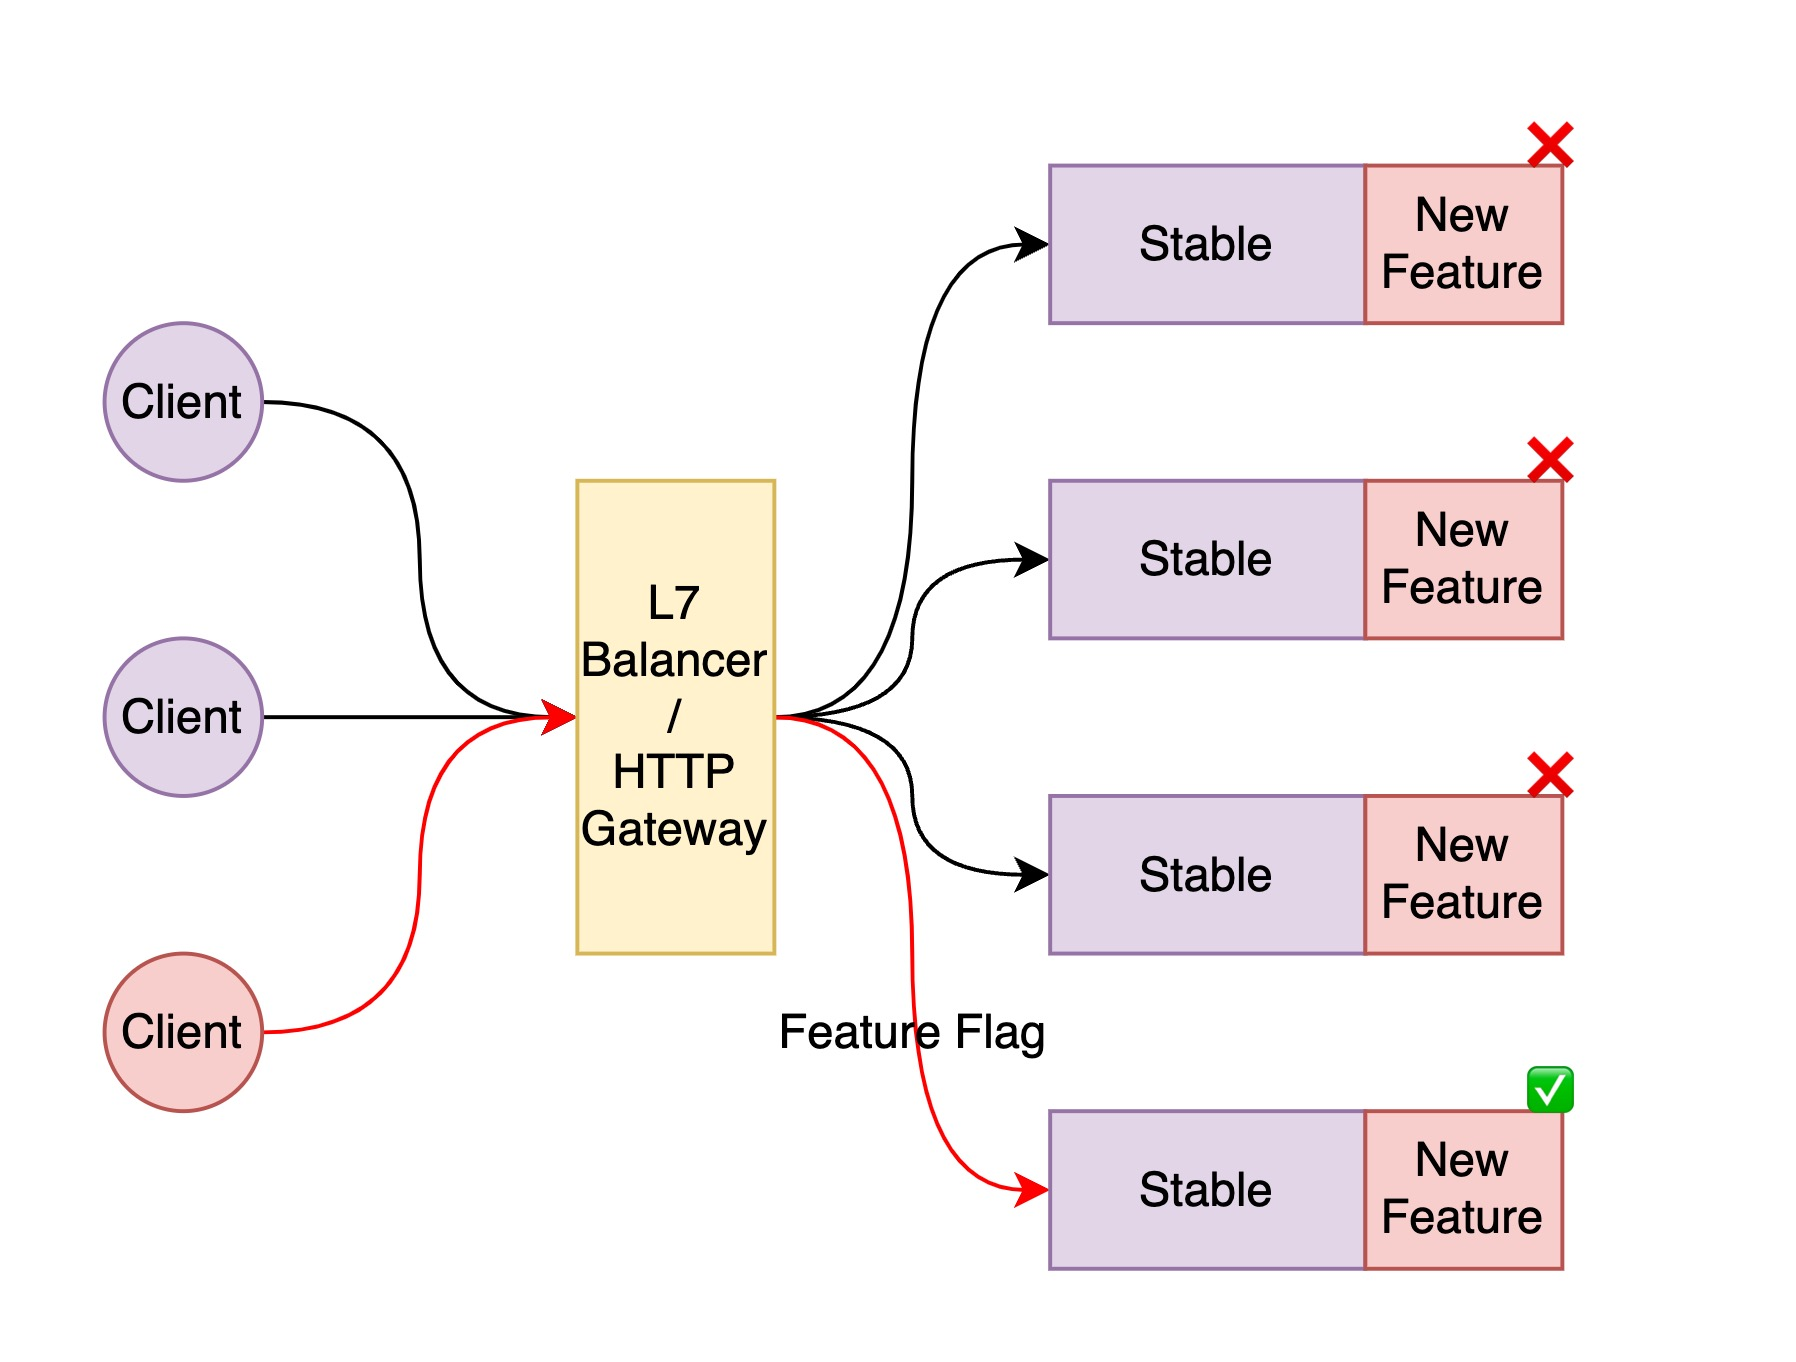
\includegraphics[width=0.8\linewidth]{img/ab.jpg}
    \caption{--- Принцип AB-тестирования}
    \label{fig:ab}
\end{figure}

В рамках тестирования новой функциональности применяется также sha\-dow deployment или теневые выкладки,
при которых трафик в стабильные версии зеркалируется в отдельные экземпляры приложения со своими персистентными хранилищами,
которые могут быть воспроизведены из оригинальных данных, что помогает оценить отказоустойчивость
приложения под нагрузкой или провести инструментацию сервиса без вреда производительности (Рисунок \ref{fig:shadow}).
Примером инструментации, которая может нести в себе потенциальные проблемы с производительностью
является PGO (Profiler Guided Optimisation), который предполагает сбор широкого спектра данных о
процессорном времени, аллокации памяти, состояния рантайма и так далее, что требует накладных расходов.
Полученные данные в последующем могут быть использованы при сборке приложения для выявления сценариев
использования системы, что подсказывает компилятору, какие оптимизации можно применить.
Сбор данных о производительности приложения в отдельном контуре может помочь наладить подобный процесс, не замедляя
при этом стабильные версии приложения.
\begin{figure}[H]
    \centering
    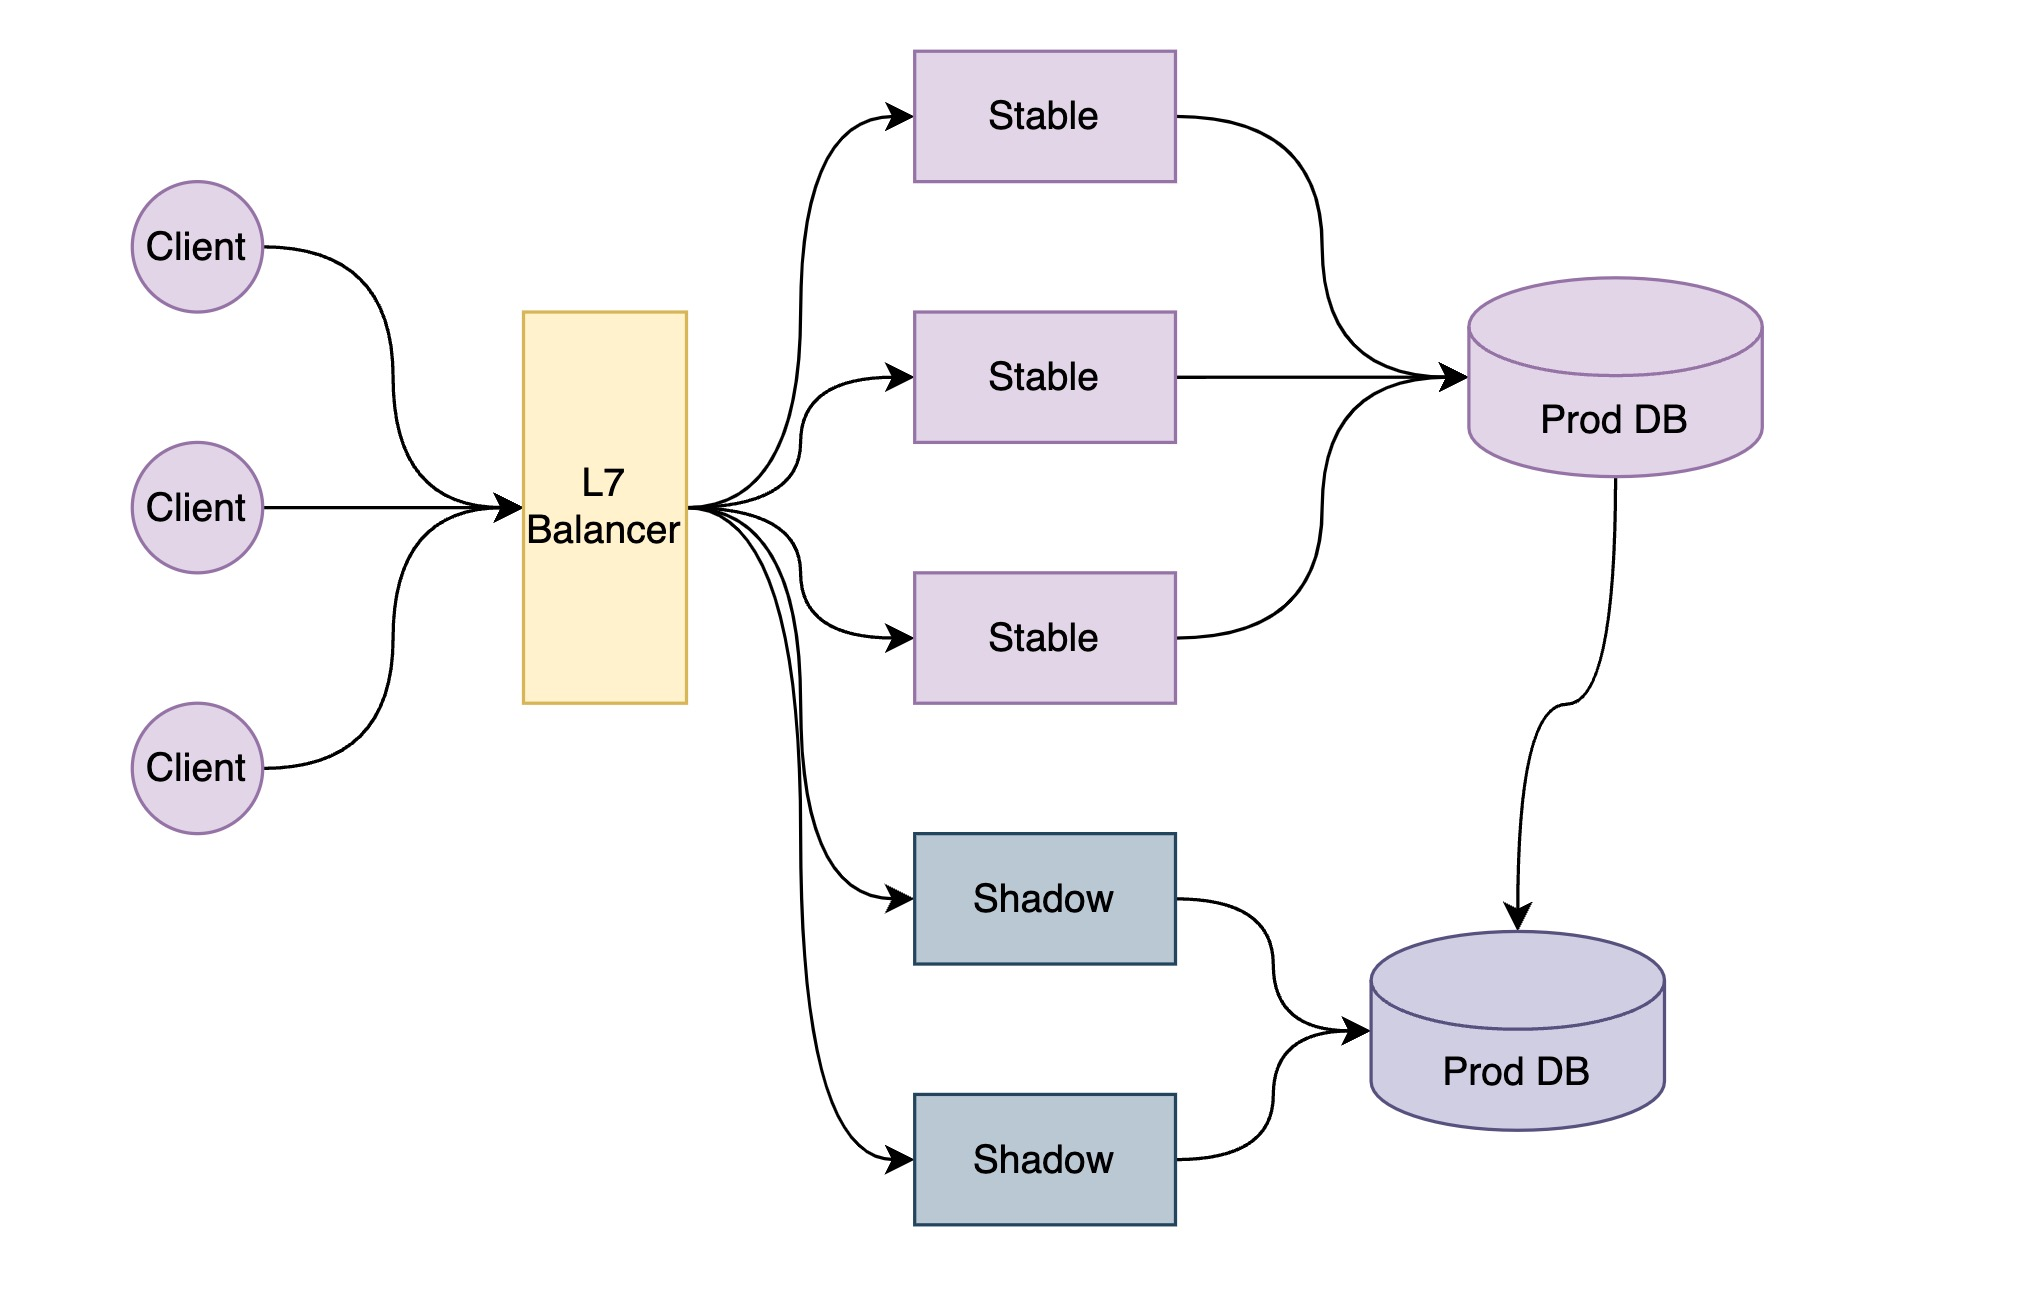
\includegraphics[width=0.8\linewidth]{img/shadow.jpg}
    \caption{--- Принцип зеркалирования трафика при shadow развертывании}
    \label{fig:shadow}
\end{figure}

В этом случае изменения можно выпускать бесперебойно и с учетом нескольких зон
доступности, что позволяет проводить инструментацию и мониторинг сервиса на самих ранних стадиях релизного цикла.

Несмотря на вышеперечисленные проблемы, при правильном распределении зон ответственности
сервисов и внедрении практик оркестрации 
релизы микросервисов могут быть проще релизов монолитных приложений, 
за счет того, что становится возможными тестировать, выкатывать 
функциональность независимо и разделить релизные циклы.

Еще одна трудность связана с решением о том, на каком этапе жизненного цикла
приложения следует переходить на микросервисную архитектуру. Часто во время
разработки первой версии система не сталкивается с проблемами, которые эта
архитектура решает \cite{kaban}. 

Применение практик микросервисного проектирования может замедлить разработку
на начальных стадиях и зачастую не несет пользы для небольших команд из-за необходимости уделять больше
внимания контрактам взаимодействия между сервисами и применении дополнительных технологий для их координации. 
Поэтому распространенной практикой является первоначальное проектирование монолитных приложений с
в возможностью последующего разделения монолита на отдельные сервисы.

Разбиение приложения на микросервисы с разными функциями может оказаться непростым
из-за запутанных зависимостей. Но обычно для сложных проектов, таких как пользовательские веб или
SaaS-приложения, это правильный выбор. Такие общеизвестные сайты, как eBay, Amazon.com, Groupon и Gilt, в свое время перешли на микросервисы с монолитной архитектуры.

При использовании микросервисов приходится иметь дело с множеством проблем, связанных с проектированием и архитектурой.
К тому же многие из этих
проблем имеют несколько решений со своими плюсами и минусами. Единого
идеального решения не существует \cite{micro-1}.

Также IDE и другие инструменты разработки рассчитаны на создание монолитных
приложений и не обеспечивают явной поддержки распределенных приложений. Зачастую микросервисы живут в разных репозиториях, что
требует отдельного версионирования каждого из компонентов. Для решения подобных проблем в некоторых системах сборки прибегают к использованию
воркспейсов, где исходные коды общего кода берутся вне зависимости от релизного цикла микросервисов, а из локальной версии репозитория,
что может облегчить локальную разработку. Однако не всегда разные микросервисы размещаются в разных репозиториях и возникает вопрос
масштабирования инфраструктуры для сборки, тестирования и разработки всего приложения. Репозитории с большим количеством независимых сервисов, но
общими версиями внешних зависимостей зачастую называют монорепозиториями. В монорепозитории инструменты сборки не всегда работают оптимально
без дополнительной конфигурации и эвристик, направленных на кэширование артефактов сборки, однако данные недостатки сопровождаются потенциальными
достоинствами в виде переиспользования кода, повышенной безопасности за счет централизации зависимостей.

